\documentclass{beamer}
\usepackage{amsmath}
\usepackage{graphicx}


\usepackage{listings}
\usepackage{color}

\definecolor{dkgreen}{rgb}{0,0.6,0}
\definecolor{gray}{rgb}{0.5,0.5,0.5}
\definecolor{mauve}{rgb}{0.58,0,0.82}

\lstset{frame=tb,
  language=Java,
  aboveskip=3mm,
  belowskip=3mm,
  showstringspaces=false,
  columns=flexible,
  basicstyle={\small\ttfamily},
  numbers=none,
  numberstyle=\tiny\color{gray},
  keywordstyle=\color{blue},
  commentstyle=\color{dkgreen},
  stringstyle=\color{mauve},
  breaklines=true,
  breakatwhitespace=true,
  tabsize=3
}




\graphicspath{ {./images/} }

\title{Least squares}
\subtitle{Sample Subtitle}
\author{Juan V. Vía}
\institute{}
\date{\today}

%\usetheme{lucid}
\begin{document}
% -------------------------------------------------------------------------
\frame {
	\titlepage
}
% -------------------------------------------------------------------------
\frame {
	\frametitle{Example}
	\framesubtitle{Showing why least squares}
	We have a variable $y$. We know that it's dependent of another variable $x$ in some
	way. But we don't know how, exactly.

	So we go to the field and measure certain points. Those that we can reach. Six of them.
	$$(2,5),(5,5),(7,8),(11,7),(14,9),(18,7)$$

	That is: at $x=2$ we measure $y=5$, at $x=5$ we measure $y=5$ again, but
	at $x=7$ we got $y=8$, and so on.
}
% -------------------------------------------------------------------------
\frame {
	\frametitle{Example}
	\framesubtitle{Showing why least squares}
	Next step, obviously, is to plot these points.
	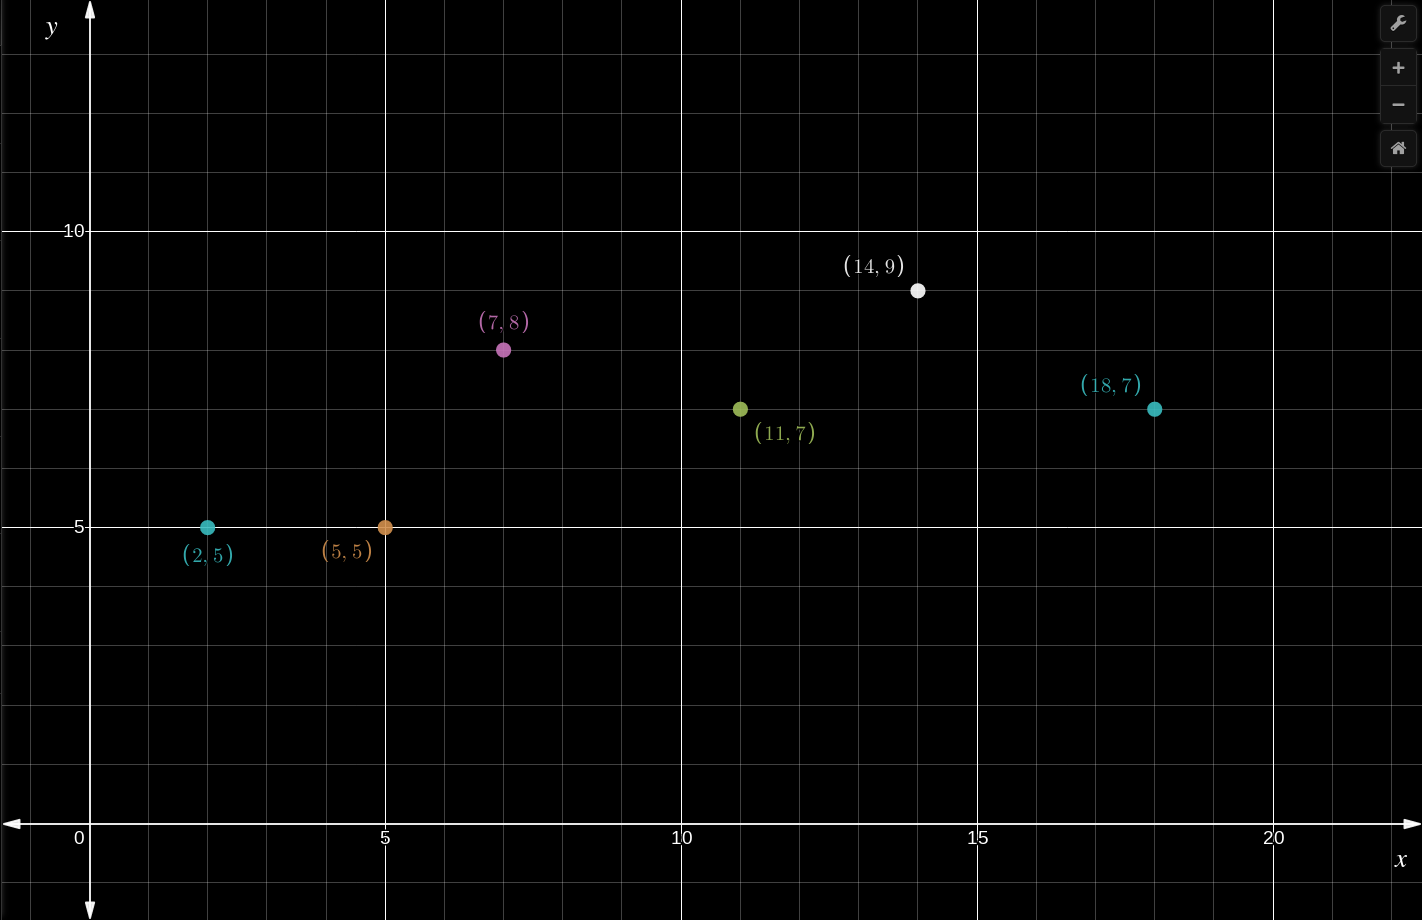
\includegraphics[width=8cm]{points}
}
% -------------------------------------------------------------------------
\frame {
	\frametitle{Example}
	\framesubtitle{Showing why least squares}
	Let's start by tracing a line wich "best fit" that data
	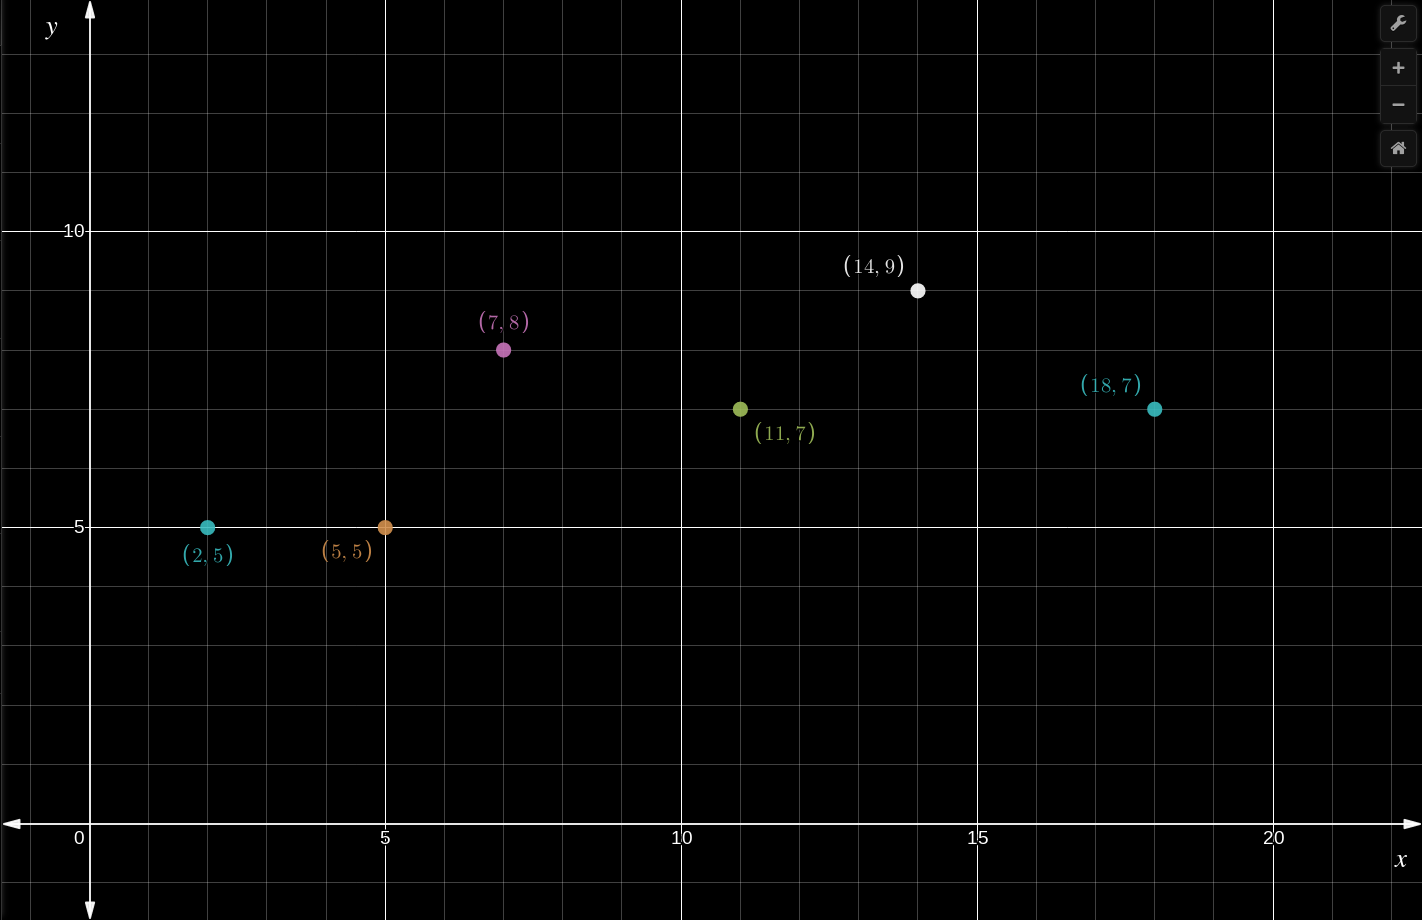
\includegraphics[width=8cm]{points}
}
% -------------------------------------------------------------------------
\frame {
	\frametitle{Example}
	\framesubtitle{Showing why least squares}
	What line? How to choose that line?
	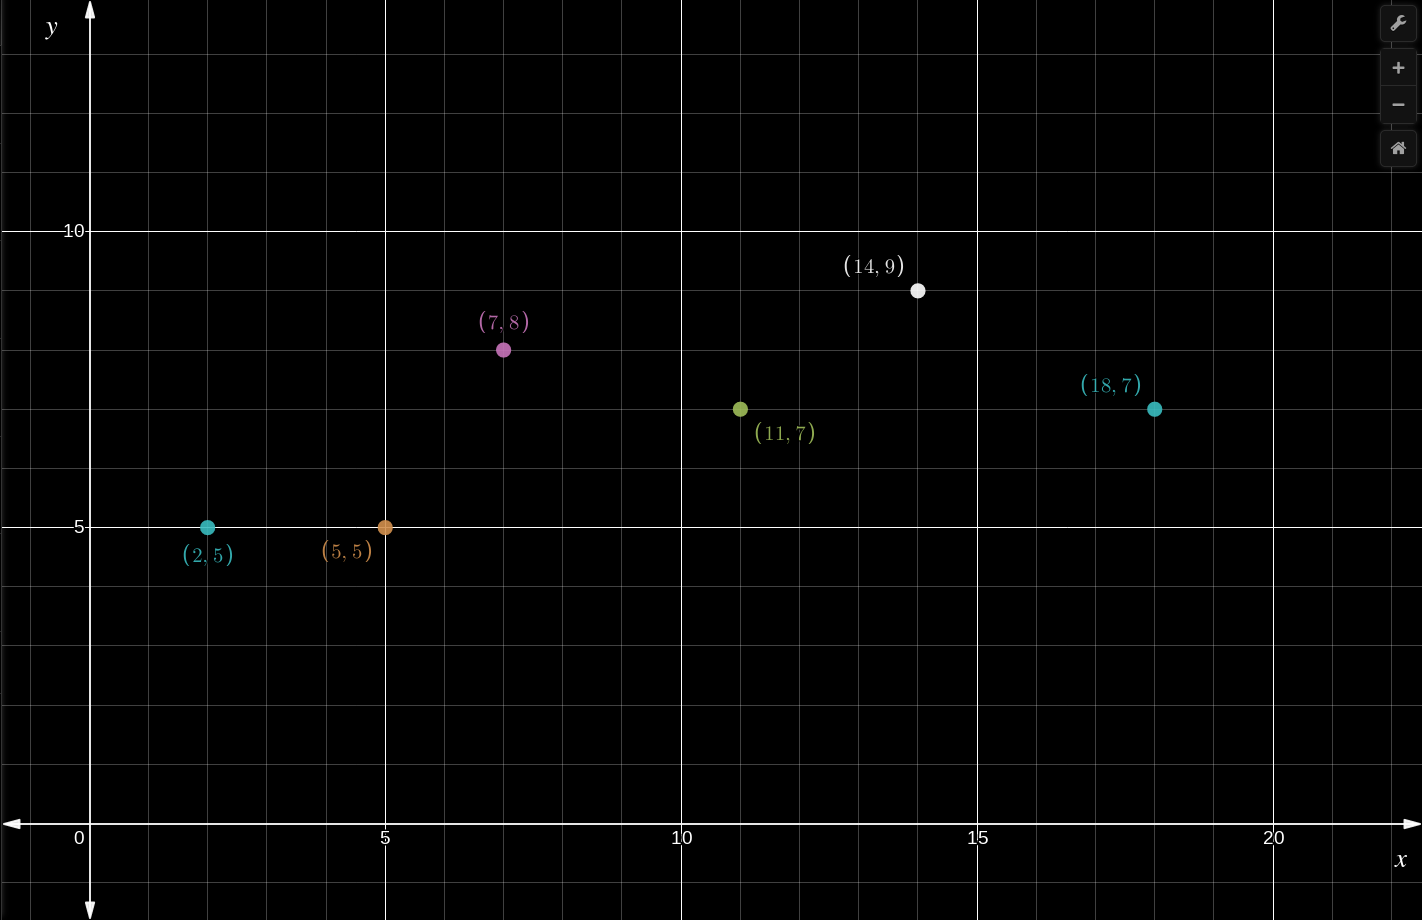
\includegraphics[width=8cm]{points}
}
% -------------------------------------------------------------------------
\frame {
	\frametitle{Example}
	\framesubtitle{Showing why least squares}

	A very common way to express a line is using the equation (a polinomial function)
	$$
		y = mx +b
	$$

	Using vector notation:
	$$y=
		\begin{bmatrix} x & 1 \end{bmatrix}
		\begin{bmatrix} m\\ b \end{bmatrix}$$

	Or, switching terms:
	$$\begin{bmatrix} x & 1 \end{bmatrix}
		\begin{bmatrix} m\\ b \end{bmatrix}=y$$
}
% -------------------------------------------------------------------------
\frame {
	\frametitle{Example}
	\framesubtitle{Showing why least squares}

	Ok. Fine. That's it. This form
	$$\begin{bmatrix} x & 1 \end{bmatrix}
		\begin{bmatrix} m\\ b \end{bmatrix}=y$$
	will be a useful one because we know $x$ and $y$ in six points.
	For example take the first point $(2,5)$
	$$\begin{bmatrix} 2 & 1 \end{bmatrix}
		\begin{bmatrix} m\\ b \end{bmatrix}=5$$
}
% -------------------------------------------------------------------------
\frame {
	\frametitle{Example}
	\framesubtitle{Showing why least squares}

	And yes, your guess is true. We can incorporate the second point $(5,5)$ and get
	$$\begin{bmatrix} 2 & 1 \\
                5 & 1\end{bmatrix}
		\begin{bmatrix} m\\ b \end{bmatrix}=\begin{bmatrix} 5\\ 5 \end{bmatrix}$$

	...and the third point...and the fourth...
}
% -------------------------------------------------------------------------
\frame {
	\frametitle{Example}
	\framesubtitle{Showing why least squares}

	Reaching the end this is the result
	$$\begin{bmatrix} 2  & 1 \\
                5  & 1 \\
                7  & 1 \\
                11 & 1 \\
                14 & 1 \\
                18 & 1
		\end{bmatrix}
		\begin{bmatrix} m\\ b \end{bmatrix}=\begin{bmatrix}
			5 \\
			5 \\
			8 \\
			7 \\
			9 \\
			7
		\end{bmatrix}$$
}
% -------------------------------------------------------------------------
\frame {
	\frametitle{Example}
	\framesubtitle{Showing why least squares}

	Time to name things.

}
% -------------------------------------------------------------------------
\frame {
	\frametitle{Example}
	\framesubtitle{Showing why least squares}

	Call $A$ to the matrix 	$$A=\begin{bmatrix}
			2  & 1 \\
			5  & 1 \\
			7  & 1 \\
			11 & 1 \\
			14 & 1 \\
			18 & 1
		\end{bmatrix}$$
}
% -------------------------------------------------------------------------
\frame {
	\frametitle{Example}
	\framesubtitle{Showing why least squares}

	Call $x$ to the column vector	$$x=\begin{bmatrix} m\\ b \end{bmatrix}$$
}
% -------------------------------------------------------------------------
\frame {
	\frametitle{Example}
	\framesubtitle{Showing why least squares}

	Call $b$ to the column vector	$$b=\begin{bmatrix}
			5 \\
			5 \\
			8 \\
			7 \\
			9 \\
			7
		\end{bmatrix}$$
}
% -------------------------------------------------------------------------
\frame {
	\frametitle{Example}
	\framesubtitle{Showing why least squares}

	Thus, the equation
	$$\begin{bmatrix} 2  & 1 \\
                5  & 1 \\
                7  & 1 \\
                11 & 1 \\
                14 & 1 \\
                18 & 1
		\end{bmatrix}
		\begin{bmatrix} m\\ b \end{bmatrix}=\begin{bmatrix}
			5 \\
			5 \\
			8 \\
			7 \\
			9 \\
			7
		\end{bmatrix}$$
	becomes
	$$ Ax=b $$
}
% -------------------------------------------------------------------------
\frame {
	\frametitle{Example}
	\framesubtitle{Showing why least squares}

	In other words: if you want to know the values $m$ and $b$ in the equation
	$ y = mx + b $ of the line we are searching find the $x$ such that $Ax=b$, but\dots

	\dots that equation have no solution!\dots

	...because the matrix A is tall, so $Ax=b$ is over-determined, there are more equations (m)
	than variables to choose. There is no $x$ such that the norm of the difference between Ax and b equals zero

	$$
		\left\lVert Ax-b\right\rVert \neq 0
	$$

	\textbf{We need the least squares approximate solution}


}
% -------------------------------------------------------------------------
\frame {
	\frametitle{Example}
	\framesubtitle{Showing why least squares}
	In the least squares approximate solution of $Ax=b$ we, provided that $\left\lVert Ax-b\right\rVert \neq 0$,
	select $x$ that the \textit{norm} of the \textit{residual} $r=Ax-b$ be minimal.

	It's all here: http://vmls-book.stanford.edu/ and in many other sources. The least squares
	approximate solution is very known.

	Let's see it.
}
% -------------------------------------------------------------------------
\frame {
	\frametitle{Example}
	\framesubtitle{Showing why least squares}

	All start with our equation $Ax=b$.


}
% -------------------------------------------------------------------------
% -------------------------------------------------------------------------
\frame {
	\frametitle{Example}
	\framesubtitle{Showing why least squares}

	Take $A$,
	$$
		A= \begin{bmatrix} 2  & 1 \\
                5  & 1 \\
                7  & 1 \\
                11 & 1 \\
                14 & 1 \\
                18 & 1
		\end{bmatrix}
	$$
	transpose it.
	$$
		A^\intercal=\begin{bmatrix} 2 & 5 & 7 & 11 & 14 & 18 \\
                1 & 1 & 1 & 1  & 1  & 1
		\end{bmatrix}
	$$
}
% -------------------------------------------------------------------------
% -------------------------------------------------------------------------
\frame {
	\frametitle{Example}
	\framesubtitle{Showing why least squares}

	Multiply $A^\intercal$ by $A$

	$$
		A^\intercal A = \begin{bmatrix} 2 & 5 & 7 & 11 & 14 & 18 \\
                1 & 1 & 1 & 1  & 1  & 1
		\end{bmatrix} \begin{bmatrix} 2  & 1 \\
                5  & 1 \\
                7  & 1 \\
                11 & 1 \\
                14 & 1 \\
                18 & 1
		\end{bmatrix} = \begin{bmatrix} 719 & 57 \\
                57  & 6
		\end{bmatrix}
	$$



}
% -------------------------------------------------------------------------
% -------------------------------------------------------------------------
\frame {
\frametitle{Example}
\framesubtitle{Showing why least squares}

Invert the product
$$
	(A^\intercal A)^{-1} = \begin{bmatrix} 719 & 57 \\
                57  & 6
	\end{bmatrix}^{-1} = \begin{bmatrix} \frac{2}{355}   & -\frac{19}{355}  \\
                -\frac{19}{355} & \frac{719}{1065}
	\end{bmatrix}
$$


}
% -------------------------------------------------------------------------
% -------------------------------------------------------------------------
\frame {
	\frametitle{Example}
	\framesubtitle{Showing why least squares}

	Multiply inverse and transpose
	$$
		(A^\intercal A)^{-1}A^\intercal = \begin{bmatrix} \frac{2}{355}   & -\frac{19}{355}  \\
                -\frac{19}{355} & \frac{719}{1065}
		\end{bmatrix}\begin{bmatrix} 2 & 5 & 7 & 11 & 14 & 18 \\
                1 & 1 & 1 & 1  & 1  & 1
		\end{bmatrix}
	$$
	$$
		= \begin{bmatrix} -\frac{3}{71}   & -\frac{9}{355}   & -\frac{1}{71}  & \frac{3}{355}   & \frac{9}{355}    & \frac{17}{355}    \\
                \frac{121}{213} & \frac{434}{1065} & \frac{64}{213} & \frac{92}{1065} & -\frac{79}{1065} & -\frac{307}{1065}
		\end{bmatrix}
	$$

	Let's call this product $(A^\intercal A)^{-1}A^\intercal$ the \textit{pseudo-inverse}

}
% -------------------------------------------------------------------------
% -------------------------------------------------------------------------
\frame {
	\frametitle{Example}
	\framesubtitle{Showing why least squares}

	Finally multiply the pseudo-inverse by $b$

	$$x = \begin{bmatrix} -\frac{3}{71}   & -\frac{9}{355}   & -\frac{1}{71}  & \frac{3}{355}   & \frac{9}{355}    & \frac{17}{355}    \\
                \frac{121}{213} & \frac{434}{1065} & \frac{64}{213} & \frac{92}{1065} & -\frac{79}{1065} & -\frac{307}{1065}
		\end{bmatrix}\begin{bmatrix}
			5 \\
			5 \\
			8 \\
			7 \\
			9 \\
			7
		\end{bmatrix} = \begin{bmatrix}
			\frac{61}{355} \\
			\frac{5539}{1065}
		\end{bmatrix}
	$$

}
% -------------------------------------------------------------------------
\frame {
	\frametitle{Example}
	\framesubtitle{Showing why least squares}

	That's it
	$$x = \begin{bmatrix}
			m \\
			b
		\end{bmatrix} = \begin{bmatrix}
			\frac{61}{355} \\
			\frac{5539}{1065}
		\end{bmatrix} \textnormal{or} \begin{bmatrix}
			0.171831 \\
			5.20094
		\end{bmatrix}
	$$
	and $m=0.171831$ and $b=5.20094$ and the line is
	$$
		y = 0.171831x+5.20094
	$$
}
% -------------------------------------------------------------------------
\frame {
	\frametitle{Example}
	\framesubtitle{Showing why least squares}
	And the best fit is
	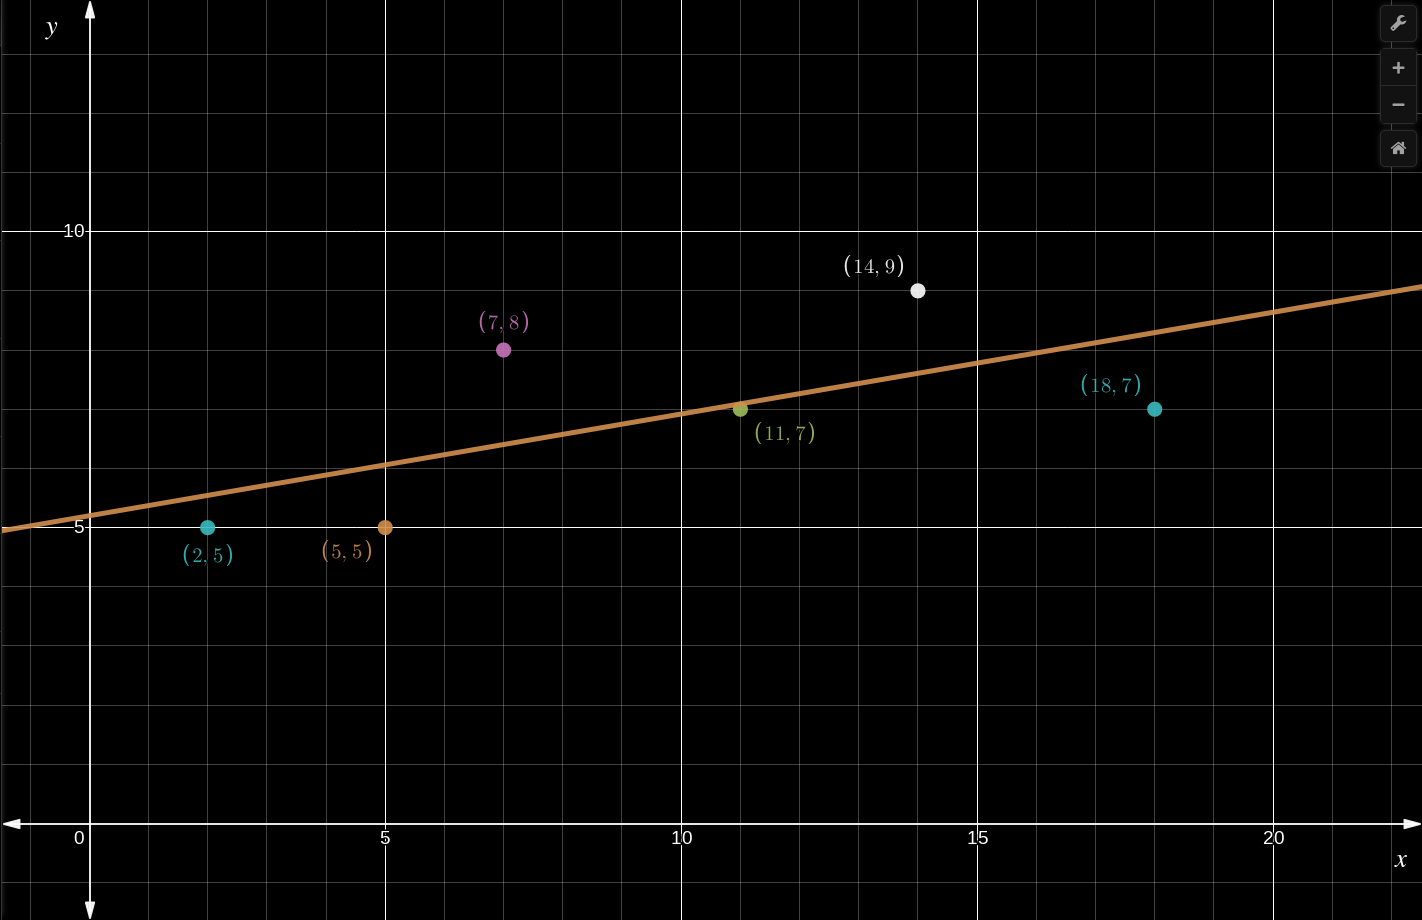
\includegraphics[width=8cm]{line}
}
% -------------------------------------------------------------------------
\frame {
	\frametitle{Least squares}
	\framesubtitle{Recapitulation}

	You have a bunch of data points and suspect that a polinomial function $y=Ax+B$ from this points is a good model.

	You build a matrix $A$ and a vector $b$ from the polinomial and the points.

	The polinomial coefficients are a vector $x$ so $Ax=b$

	Then $x=(A^\intercal A)^{-1}A^\intercal b$


}
% -------------------------------------------------------------------------
\frame {
	\frametitle{Least squares}
	\framesubtitle{Don't worry, its XXI century}

	So the solution is calculate $x=(A^\intercal A)^{-1}A^\intercal b$

	But you don't need to do this by hand like Gauss did.

	See the code, in this case Javascript code


}
% -------------------------------------------------------------------------
\begin{frame}[fragile]
\begin{lstlisting}
const { multiply, transpose, inv, matrix, format } = require( "mathjs")

const solve = (A, b) => {
	const transposed    = transpose(A)
	const product       = multiply(transposed, A)
	const inverse       = inv(product)
	const pseudoInverse = multiply(inverse,transposed)
	const x             = multiply(pseudoInverse, b)
	return x
}

const A = matrix([[2,1],[5,1],[7,1],[11,1],[14,1],[18,1]])
const b = matrix([5,5,8,7,9,7]);

console.log(format(solve(A, b),5))
\end{lstlisting}
\end{frame}
% -------------------------------------------------------------------------
\frame {
	\frametitle{Least squares}
	\framesubtitle{The polinomial function}

	In the example we picked a line for regression.

	A line in a plane is a polinomial function where $y$ (the dependent variable, a real number) is a
	function of $x$ (the independent variable, a real number)
	$$
		y \colon \mathbb{R} \to \mathbb{R} = Ax + B
	$$

}
% -------------------------------------------------------------------------
\end{document}